\documentclass[10pt,a4paper,UTF8]{article}
\usepackage{zclorg}
\author{张朝龙}
\date{}
\title{学习Python第一天}
\hypersetup{
 pdfauthor={张朝龙},
 pdftitle={学习Python第一天},
 pdfkeywords={},
 pdfsubject={},
 pdfcreator={Emacs 25.0.50.1 (Org mode 8.3.4)}, 
 pdflang={English}}
\begin{document}

\maketitle
\tableofcontents
\titlepic{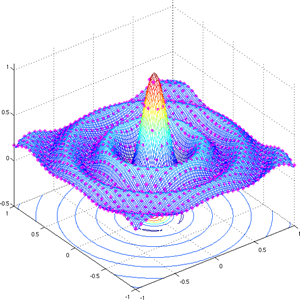
\includegraphics[scale=0.25]{../../img/sinc.PNG}}
\newpage

今天是学习Python第一天,我从其官方文档入手,\href{https://docs.python.org/3.5/tutorial/index.html}{英文版地址} \href{http://docspy3zh.readthedocs.io/en/latest/tutorial/}{中文版地址} 。在学习的过程中,我以英文版为主,参照了中文版,这一系列博文是我的学习笔记,不是严格的文档翻译,很多地方按照我的理解进行了转述,我认为每个人的第一份Python学习资料都应该是其官方文档。尽管从这个文档不可能学到所有的Python特性(要想学习到所有的Python特性需要阅读其官方手册和大量的标准库文档。),但是你学到的是最正统的Python。

我的学习环境是Windows + Anaconda + Python3.5 + Emacs. 我在Windows 上使用Emacs作为Python3.5的前端。在Emacs里使用IPython这样的REPL环境,大大提高了我的学习效率。另外为了使得报错提示显示为英文,我把Windows的语言环境改成了英文。

嗯,开始吧!

\section{Python简介}
\label{sec:orgheadline1}


Python简单易用,功能强大。相对于其他语言,它有更高级别的语言抽象和更有效的面向对象编程范式。Python的语法造就了Python程序格式上的优美,对于强迫症患者来说是福音。Python的解释特性使其成为脚本语言和快速开发部署的绝佳选择。

从\href{https://www.python.org/}{Python的官网}上, 可以获得Python解释器和更多的第三方扩展库。当然,Python自带功能强大的\href{https://docs.python.org/3.5/library/index.html#library-index}{标准库} 。Python的解释器使其可以方便的\href{https://docs.python.org/3.5/extending/index.html#extending-index}{同其他语言(C/C++)进行扩展} ,从而强化了Python的可扩展性。

\section{人生苦短,Python必选。}
\label{sec:orgheadline2}


每个人都有自动化大量重复性劳动的冲动。因为重复性的劳动让人大脑迟钝,生活变得索然无味。在不停的重复过程中,生命就这么浪费了。Python会以出人意料的速度帮你完成重复性劳动,让你有时间去爬山。 如果你是一个程序员,肯定发现C/C++这类语言在编写代码编译代码重新编译代码的循环中浪费了好多青春。即便程序最终可以运行,为这个程序写大量的测试用例也要占用不少时间。

人生苦短,Python必选。

Python提供了不但Unix shell一样的批处理,还提供了可移植性。Python允许你的代码高度解耦,模块的重用易如反掌。Python本身携带了大量的标准模块,任君选择。作为一门解释性语言,Python不需要编译和链接,解释器也可以交互式的实用,随时查看程序结果。

\section{上手Python解释器}
\label{sec:orgheadline3}


这里我就不废话怎么安装Python环境了。我的IPyton启动后画面是:
\begin{figure}[htb]
\centering
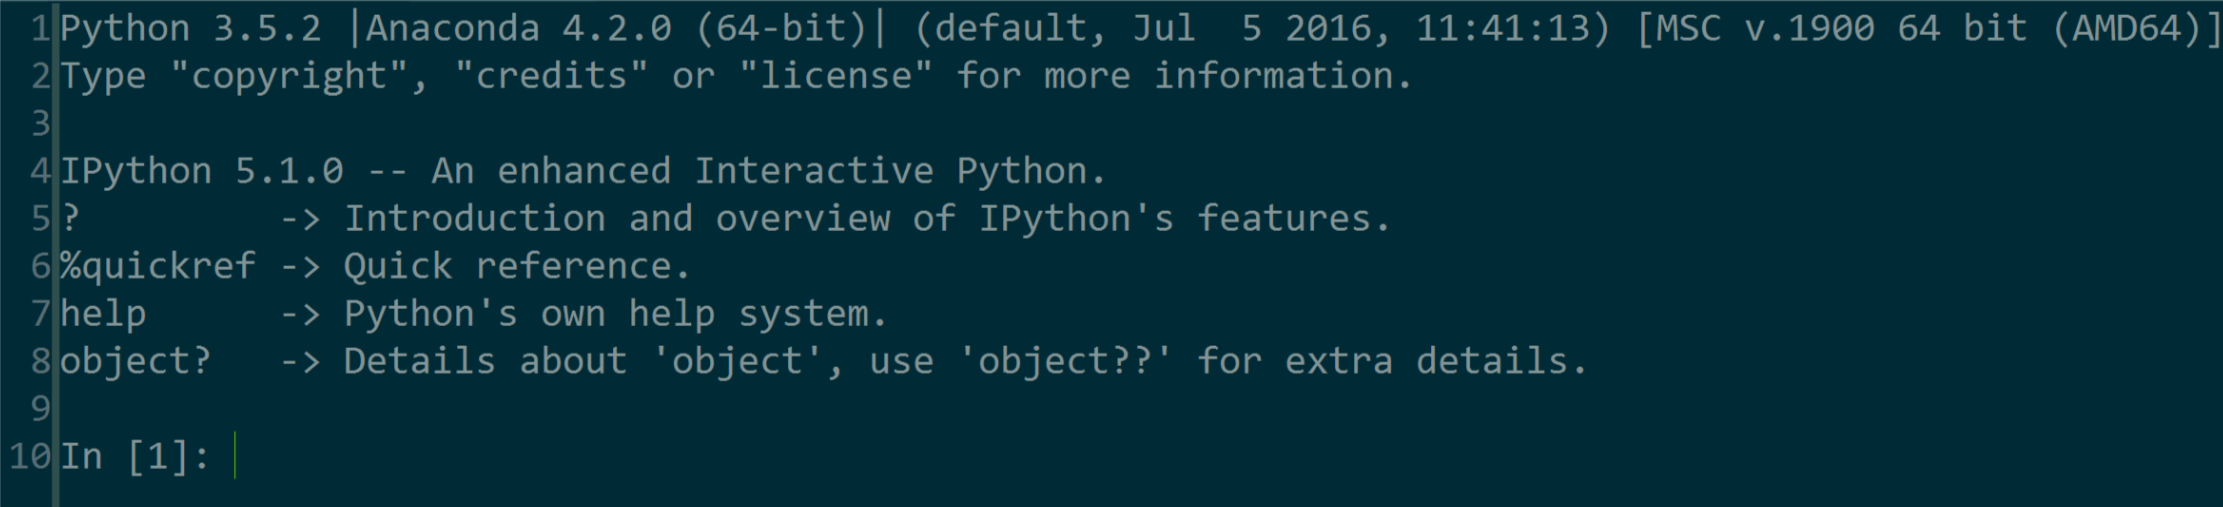
\includegraphics[width=0.6\textwidth]{../../img/20170312PythonDay01.PNG}
\caption{\label{fig:orgparagraph1}
我的Python启动画面}
\end{figure}

Python文件默认编码方式是 \texttt{UTF-8} 。可以在文件头部添加: 
\begin{verbatim}
# -*- coding: UTF-8 -*-
\end{verbatim}
指定源文件采用 \texttt{UTF-8} 编码。在Python中使用 \texttt{\#} 作为注释开始标志。

\section{把Python当计算器用}
\label{sec:orgheadline7}


\subsection{数值计算}
\label{sec:orgheadline4}
\lstset{language=Python,label= ,caption= ,captionpos=b,numbers=none}
\begin{lstlisting}
In [28]: 2/7 
Out[42]: 
0.2857142857142857

In [43]: 50 - 9/6
Out[59]: 
48.5
In [60]:
\end{lstlisting}

整数 \texttt{2,4,9} 类型是 \texttt{int} ;有小数点的数 \texttt{48.5} 类型是 \texttt{float} ; 除法计算 \texttt{/} 总是返回浮点数。 为舍弃小数点部分,需要使用 \texttt{//} , 示例:
\lstset{language=Python,label= ,caption= ,captionpos=b,numbers=none}
\begin{lstlisting}
In [60]: 17/3
Out[67]: 
5.666666666666667

In [68]: 17//3
Out[78]: 
5
\end{lstlisting}

可以看出 \texttt{//} 进行的不是四舍五入,是直接舍弃小数部分,只保留整数部分。

Python使用 \texttt{**} 完成幂计算,示例:
\lstset{language=Python,label= ,caption= ,captionpos=b,numbers=none}
\begin{lstlisting}
In [82]: 2**10
Out[92]: 1024

In [93]: 3**8
Out[100]:6561
\end{lstlisting}

\texttt{=} 号的一个作用是变量赋值,示例:
\lstset{language=Python,label= ,caption= ,captionpos=b,numbers=none}
\begin{lstlisting}
In [101]: width = 20

In [109]: height = 5*9

In [117]: width * height
Out[128]: 
900
\end{lstlisting}
如果变量没有被定义,会报错,示例:
\lstset{language=Python,label= ,caption= ,captionpos=b,numbers=none}
\begin{lstlisting}
In [129]: n
---------------------------------------------------------------------------
NameError                                 Traceback (most recent call last)
<ipython-input-133-fe13119fb084> in <module>()
----> 1 n

NameError: name 'n' is not defined
\end{lstlisting}

当整型和浮点类型一起混合使用时,结果为浮点类型:
\lstset{language=Python,label= ,caption= ,captionpos=b,numbers=none}
\begin{lstlisting}
In [134]: 3 * 3.75/1.5
Out[153]: 
7.5
\end{lstlisting}
在交互式环境中,最后一个打印的表达式可以用 \texttt{\_} 来表示:
\lstset{language=Python,label= ,caption= ,captionpos=b,numbers=none}
\begin{lstlisting}
In [154]: tax = 12.5/100

In [176]: price = 100.50

In [187]: price*tax
Out[194]: 
12.5625

In [195]: price + _
Out[205]: 
113.0625

In [206]: round(_,2)
Out[212]: 
113.06
\end{lstlisting}

除了 \texttt{int} 和 \texttt{float} , Python 支持也其他类型的数据,比如 \texttt{Decimal} 和 \texttt{Fraction} 。另外Python内置复数类型比如 \texttt{3+5j}
\lstset{language=Python,label= ,caption= ,captionpos=b,numbers=none}
\begin{lstlisting}
In [213]: n= 3+5i
  File "<ipython-input-220-1c979fa6598a>", line 1
    n= 3+5i
          ^
SyntaxError: invalid syntax


In [221]: n = 3+5j

In [233]: abs(n)
Out[233]: 
5.830951894845301
\end{lstlisting}
注意是 \texttt{3+5j} 而不是 \texttt{3+5i} .

\subsection{字符串}
\label{sec:orgheadline5}


Python的字符串可以使用单引号 ='\ldots{}'= 也可以使用双引号 ="\ldots{}"= 。使用 \texttt{\textbackslash{}} 做转义字符。
\lstset{language=Python,label= ,caption= ,captionpos=b,numbers=none}
\begin{lstlisting}
In [234]: 'span eggs'
Out[249]: 
'span eggs'

In [250]: 'doesn\'t'
Out[278]: 
"doesn't"

In [279]: "doesn't"
Out[291]: 
"doesn't"

In [292]: '"Yes," he said.'
Out[312]: 
'"Yes," he said.'

In [313]: "\"Yes,\" he said."
Out[333]: 
'"Yes," he said.'

In [334]: '"Isn\'t," she said.'
Out[368]: 
'"Isn\'t," she said.'
\end{lstlisting}

在交互式环境中,字符串的输出使用双引号;特殊字符使用反斜杠保留。 \texttt{print()} 函数打印的结果更具可读性:
\lstset{language=Python,label= ,caption= ,captionpos=b,numbers=none}
\begin{lstlisting}
In [334]: '"Isn\'t," she said.'
Out[368]: 
'"Isn\'t," she said.'

In [369]: print('"Isn\'t," she said')
"Isn't," she said

In [402]: s = 'First line.\nSecond line.'

In [441]: print(s)
First line.
Second line.
\end{lstlisting}
如果你不希望 \texttt{print()} 中 \texttt{\textbackslash{}} 转义,可以使用 \texttt{r} 选项:
\lstset{language=Python,label= ,caption= ,captionpos=b,numbers=none}
\begin{lstlisting}
In [446]: print("C:\some\name")
C:\some
ame

In [466]: print(r"C:\some\name")
C:\some\name
\end{lstlisting}
Python 使用 ="""\ldots{}"""= 支持多行字符:
\lstset{language=Python,label= ,caption= ,captionpos=b,numbers=none}
\begin{lstlisting}
print("""
This is a
string
occupying multiple lines
""")
\end{lstlisting}
输出:
\begin{verbatim}
In [487]: 
This is a
string
occupying multiple lines
\end{verbatim}
也可以使用 \texttt{+} 级联多个字符串。
\lstset{language=Python,label= ,caption= ,captionpos=b,numbers=none}
\begin{lstlisting}
In [518]: 4*"love " + "u"
Out[518]: 
'love love love love u'
\end{lstlisting}

多个字符串放在一起也可以实现自动级联:
\lstset{language=Python,label= ,caption= ,captionpos=b,numbers=none}
\begin{lstlisting}
In [519]: "python" "is" 'good'
Out[547]: 
'pythonisgood'
\end{lstlisting}

但是这样的方式只支持字符串级联,不支持变量和字符串级联:
\lstset{language=Python,label= ,caption= ,captionpos=b,numbers=none}
\begin{lstlisting}
In [548]: prefix = 'py'

In [561]: prefix 'thon'
  File "<ipython-input-570-37b5e5a6971f>", line 1
    prefix 'thon'
                ^
SyntaxError: invalid syntax
\end{lstlisting}
如果要变量和字符串级联,需要使用 \texttt{+} :
\lstset{language=Python,label= ,caption= ,captionpos=b,numbers=none}
\begin{lstlisting}
In [571]: prefix + 'thon'
Out[587]: 
'python'
\end{lstlisting}

可以使用下表来索引字符串中的字符:
\lstset{language=Python,label= ,caption= ,captionpos=b,numbers=none}
\begin{lstlisting}
In [626]: word = 'python'

In [643]: word[0]
Out[654]: 
'p'

In [655]: word[6]
---------------------------------------------------------------------------
IndexError                                Traceback (most recent call last)
<ipython-input-658-9f3bdf74c108> in <module>()
----> 1 word[6]

IndexError: string index out of range

In [659]: word[5]
Out[662]: 
'n'
\end{lstlisting}

注意下标索引和 \texttt{C/C++} 一样从 \texttt{0} 开始,并且不能越界。除了这种索引方式, Python 提供了从后面倒着索引的方法:
\lstset{language=Python,label= ,caption= ,captionpos=b,numbers=none}
\begin{lstlisting}
In [663]: word[-1]
Out[674]: 
'n'

In [675]: word[-5]
Out[684]: 
'y'

In [685]: word[-6]
Out[688]: 
'p'

In [689]: word[-7]
---------------------------------------------------------------------------
IndexError                                Traceback (most recent call last)
<ipython-input-699-03d2d1c3cbaf> in <module>()
----> 1 word[-7]

IndexError: string index out of range
\end{lstlisting}

注意倒着索引也有越界的问题。

除了逐个索引单字符,索引字符串中的某几个部分也是可以的:
\lstset{language=Python,label= ,caption= ,captionpos=b,numbers=none}
\begin{lstlisting}
In [700]: word[0:2]
Out[703]: 
'py'

In [704]: word[3:5]
Out[714]: 
'ho'
\end{lstlisting}
注意部分索引时,冒号前面的索引号是包含的,冒号后面的索引号是不包含的, \texttt{n:N} 的含义是:从第 \texttt{n} (包括) 到第 \texttt{N} (不包括)。

\lstset{language=Python,label= ,caption= ,captionpos=b,numbers=none}
\begin{lstlisting}
In [715]: word[:2] + word[2:]
Out[738]: 
'python'

In [739]: word[:5] + word[5:]
Out[751]: 
'python'
\end{lstlisting}

Python 不允许修改字符串,如果你需要一个新的字符,重新创建一个:
\lstset{language=Python,label= ,caption= ,captionpos=b,numbers=none}
\begin{lstlisting}
In [752]: word[0] = 'J'
--------------------------------------------------------------
TypeError                    Traceback (most recent call last)
<ipython-input-771-197b67ffdd83> in <module>()
----> 1 word[0] = 'J'

TypeError: 'str' object does not support item assignment


In [772]: 'J' + word[1:]
Out[778]: 
'Jython'
\end{lstlisting}
内置的 \texttt{len()} 函数返回字符串的长度:
\lstset{language=Python,label= ,caption= ,captionpos=b,numbers=none}
\begin{lstlisting}
In [779]: s = 'askkjljlkjioejkjlkjlskjlj'

In [793]: len(s)
Out[801]: 
25
\end{lstlisting}
\subsection{列表(list)}
\label{sec:orgheadline6}

Python支持很多复杂的数据类型,列表(list)是比较常用的一个:

\lstset{language=Python,label= ,caption= ,captionpos=b,numbers=none}
\begin{lstlisting}
In [802]: squares = [1,4,9,16,25]

In [833]: squares
Out[837]: 
[1, 4, 9, 16, 25]
\end{lstlisting}
就像字符串一样,列表也可以用下表正向索引或者逆向索引
\lstset{language=Python,label= ,caption= ,captionpos=b,numbers=none}
\begin{lstlisting}
In [890]: squares[-2:1]
Out[900]: 
[]

In [901]: squares[-2:-4]
Out[901]: 
[]

In [902]: squares[2:4]
Out[902]: 
[9, 16]

In [903]: squares[-4:-2]
Out[909]: 
[4, 9]
\end{lstlisting}
list支持级联:
\lstset{language=Python,label= ,caption= ,captionpos=b,numbers=none}
\begin{lstlisting}
In [910]: squares + [36,49,64,81,100]
Out[952]: 
[1, 4, 9, 16, 25, 36, 49, 64, 81, 100]
\end{lstlisting}
不像字符串不能被修改,list是可以修改的:
\lstset{language=Python,label= ,caption= ,captionpos=b,numbers=none}
\begin{lstlisting}
In [953]: cubes = [1, 8, 27,65,125]

In [988]: cubes[3] = 64

In [1000]: cubes
Out[1004]: 
[1, 8, 27, 64, 125]
\end{lstlisting}

可以使用 \texttt{append()} 方法向list的尾巴上追加数据:
\lstset{language=Python,label= ,caption= ,captionpos=b,numbers=none}
\begin{lstlisting}
In [1000]: cubes
Out[1004]: 
[1, 8, 27, 64, 125]

In [1005]: cubes.append(216)

In [1020]: cubes.append(7**3)

In [1038]: cubes
Out[1038]: 
[1, 8, 27, 64, 125, 216, 343]
\end{lstlisting}

list也可以部分索引:
\lstset{language=Python,label= ,caption= ,captionpos=b,numbers=none}
\begin{lstlisting}
In [1039]: letters = ['a','b','c','d','e','f','g','h']

In [1075]: letters
Out[1075]: 
['a', 'b', 'c', 'd', 'e', 'f', 'g', 'h']

In [1076]: #replace some values

In [1081]: letters[2:5] = ['C','D','E']

In [1095]: letters
Out[1095]: 
['a', 'b', 'C', 'D', 'E', 'f', 'g', 'h']

In [1096]: #now remove them

In [1108]: letters[2:5] = []

In [1115]: letters
Out[1123]: 
['a', 'b', 'f', 'g', 'h']

In [1124]: # clear all items

In [1136]: letters[:] = []

In [1147]: letters
Out[1147]: 
[]
\end{lstlisting}
内置的 \texttt{len()} 函数同样返回list的长度。

可以嵌套list:
\lstset{language=Python,label= ,caption= ,captionpos=b,numbers=none}
\begin{lstlisting}
In [1148]: a = ['a','b','c']

In [1157]: n = [1,2,3]

In [1168]: x = [a,n]

In [1177]: x
Out[1181]: 
[['a', 'b', 'c'], [1, 2, 3]]

In [1182]: x[0]
Out[1189]: 
['a', 'b', 'c']

In [1190]: x[1]
Out[1190]: 
[1, 2, 3]

In [1191]: len(x)
Out[1195]: 
2

In [1196]: len(x[0])
Out[1207]: 
3
\end{lstlisting}
\section{跨出编程的第一步}
\label{sec:orgheadline8}


Python能做的事情可不止一个计算器那么简单。看下面的小例子:
\lstset{language=Python,label= ,caption= ,captionpos=b,firstnumber=1,numbers=left}
\begin{lstlisting}
# Fibonacci series:
# the sum of two elements defines the next
a,b = 0,1
while b<10:
    print(b)
    a,b = b,a+b
\end{lstlisting}
输出为:
\begin{verbatim}
1
1
2
3
5
8
\end{verbatim}

解读一下上面的程序:
\begin{enumerate}
\item 第一行和第二行是注释,第三行执行了多变量赋值操作。变量 \texttt{a} 和 \texttt{b} 同时被赋值为 \texttt{0} 和 \texttt{1} 。第6行也用了多变量赋值操作。
\item \texttt{while} 循环会一直循环下去, 只要 \texttt{(b<10)} 为真。在Python中,任何非零的值都会被当做true来处理,但是在Java中 true和false是boolean类型。所以Python语言是一种比Java对类型约束比较弱的语言,可以说是弱类型语言。
\item \texttt{while} 的内容通过缩进表示。
\item 可以使用 \texttt{end} 来避免 \texttt{print()} 函数生成新行
\end{enumerate}

\lstset{language=Python,label= ,caption= ,captionpos=b,numbers=none}
\begin{lstlisting}
#+begin_src python -n
# Fibonacci series:
# the sum of two elements defines the next
a,b = 0,1
while b<10:
    print(b,end = ',')
    a,b = b,a+b
\end{lstlisting}
输出为:
\begin{verbatim}
1,2,3,5,8
\end{verbatim}
\end{document}
